% Sandia National Laboratories is a multimission laboratory managed and
% operated by National Technology & Engineering Solutions of Sandia, LLC, a
% wholly owned subsidiary of Honeywell International Inc., for the U.S.
% Department of Energy’s National Nuclear Security Administration under
% contract DE-NA0003525.

% Copyright 2002-2025 National Technology & Engineering Solutions of Sandia,
% LLC (NTESS).

%%-------------------------------------------------------------------------
%% Purpose        : Main LaTeX Xyce Users' Guide
%% Special Notes  : Graphic files (pdf format) work with pdflatex.  To use
%%                  LaTeX, we need to use postcript versions.  Not sure why.
%% Creator        : Eric keiter
%% Creation Date  : 08/26/2007
%%
%%-------------------------------------------------------------------------

% -------------------------------------------------------------------------
% Initial Condition specifications Chapter --------------------------------
% -------------------------------------------------------------------------

\chapter{Specifying Initial Conditions}
\label{IC_Chap}

\index{Initial Conditions}

\chapteroverview{Chapter Overview}
{
This chapter includes the following sections:
\begin{XyceItemize}
\item Section~\ref{IC_Overview}, {\em Initial Conditions Overview}
\item Section~\ref{IC_equals_spec}, {\em Device Level IC= Specification}
\item Section~\ref{IC_statement_spec}, {\em .IC and .DCVOLT Initial Condition Statements}
\item Section~\ref{NODESET_statement_spec}, {\em .NODESET Initial Condition Statements}
\item Section~\ref{SAVE_statement_spec}, {\em .SAVE Statements}
\item Section~\ref{UIC_NOOP_spec}, {\em UIC and NOOP}
\end{XyceItemize}
}

\section{Initial Conditions Overview}
\label{IC_Overview}

\Xyce{} provides several different options for users to set an initial
condition. Reasons for setting initial conditions include, but are not
limited to:

\begin{XyceItemize}
\item Improving the robustness of the DCOP solution
\item Optimizing performance by reusing a DCOP solution of a previous run to start new transient runs
\item Setting an initial state for a digital circuit
\item Initiating an oscillator circuit.
\end{XyceItemize}

As noted, setting initial conditions can be particularly useful for multistate
digital circuits.  Figure~\ref{preset_vs_nopreset} provides an example result demonstrating how initial conditions can be used 
to set the state of a digital circuit.
In this case, obtaining the state purely through transient simulation can be time-consuming and often is not practical..  

%  no-preset
\begin{figure}[ht]
  \centering
  \scalebox{0.5}
  { 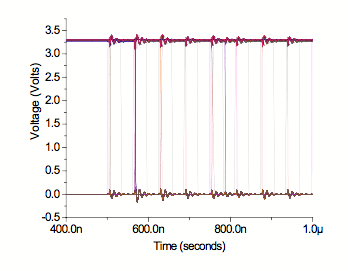
\includegraphics{preset} 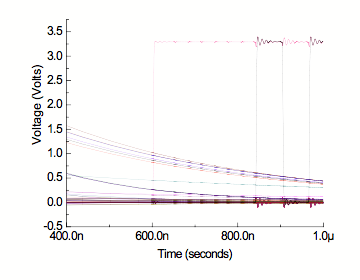
\includegraphics{nopreset} }
  \caption[Example result with and without an Initial Condition (IC).]
  {Example result with (left) and without (right) an IC on the output.  
NOTE:	The preset example, with an IC, starts in the initial state directly out of the DCOP calculation, while the non-preset example requires a long transient to equilibrate.  \label{preset_vs_nopreset}}
\end{figure}

\newpage
\section{Device Level IC= Specification}
\label{IC_equals_spec}

\index{IC=}

Many devices in \Xyce{} support setting initial junction voltage
conditions on the device instance line with the \texttt{IC=} keyword.
This is frequently used to set the state of digital circuits.
Figure~\ref{IC_Netlist_1} presents a simple inverter example
demonstrating the use of \texttt{IC=} on a BSIMSOI device.  In this
example, the two initial conditions are specified as a vector, which is the
preferred syntax.  The initial conditions can also be specified separately
(e.g., \texttt{IC1=}2  \texttt{IC2=}0).

While many circuit simulators have a similar \texttt{IC=} capability,
\Xyce{} implementation differs in some important respects.  For any
device with an \texttt{IC=} statement, \Xyce{} enforces the junction
drop during the operating point computation by inserting a voltage
source in parallel with the device junction.  \Xyce{} then applies the
parallel voltage source through the DCOP calculation, and then removes
it prior to the beginning of the transient.  This strongly enforces
the requested junction drop, meaning that if the DCOP converges, the
requested voltage drop will be in the solution and the entire circuit
solution will be consistent with that voltage drop.  Many other
circuit codes apply \texttt{IC=} as a weaker constraint, with the
intent of improving DCOP calculation robustness.

\texttt{IC=} can be applied to the following devices:  BSIM3, BSIM4, BSIMSOI,
Capacitor, Inductor and Digital Behavioral Devices (U and Y).

In the case of the capacitor, initial conditions specified via an
\texttt{IC=} parameter are also applied as an initial condition for
transients in the case that the user has used a \texttt{NOOP} or
\texttt{UIC} option on a transient line, bypassing the operating point
calculation.  In this case only, the initial condition is not enforced by
the addition of a voltage source, but rather by a weaker constraint
similar to the method used by other SPICE-type simulators.

\begin{figure}[htbp]
\begin{centering}
\shadowbox{
\begin{minipage}{0.8\textwidth}
\begin{vquote}
MOS LEVEL=10 INVERTER WITH IC=

.subckt INV IN OUT VDD GND
MN1 OUT IN GND GND GND NMOS w=4u  l=0.15u \color{XyceRed}IC=2,0 \color{black}
MP1 OUT IN VDD GND VDD PMOS w=10u l=0.15u 
.ends

.tran 20ns 30us
.print tran v(vout) {v(in)+1.0} v(1)

VDDdev  VDD 0 2V
RIN IN  1 1K
VIN1  1 0  2V PULSE (2V 0V 1.5us 5ns 5ns 1.5us 3.01us)
R1    VOUT  0  10K
C2    VOUT  0  0.1p
XINV1 IN VOUT VDD 0 INV
.MODEL NMOS NMOS ( LEVEL = 10 )
.MODEL PMOS PMOS ( LEVEL = 10 )

.END
\end{vquote}
\end{minipage}
}
\caption[Example netlist with device-level IC=.]{Example netlist with device-level IC=.\label{IC_Netlist_1}}
\end{centering}
\end{figure}

\newpage
\section{.IC and .DCVOLT Initial Condition Statements}
\label{IC_statement_spec}

\index{\texttt{.IC}}
\index{\texttt{.DCVOLT}}

\texttt{.IC} and \texttt{.DCVOLT} are equivalent methods for
specifying initial conditions.  How \Xyce{} applies them, however,
depends on whether the \texttt{UIC} parameter, discussed in a following
subsection, is present on the \texttt{.TRAN} line.  
If \texttt{UIC} is not specified, then \Xyce{}
applies the conditions specified by \texttt{.IC} and
\texttt{.DCVOLT} statements throughout the DCOP phase, ensuring the
specified values will be the solved values at the end of the DCOP
calculation.  \Xyce{} allows unspecified variables to find their
computed values, consistent with the imposed voltages.

\begin{figure}[htbp]
\begin{centering}
\shadowbox{
\begin{minipage}{0.8\textwidth}
\begin{vquote}
RC circuit
\color{XyceRed}.ic v(1)=1.0\color{black}
c1 1 0 1uF 
R1 1 2 1K
v1 2 0 0V
.print tran v(1)
.tran 0 5ms
.options timeint reltol=1e-6 abstol=1e-6
.end
\end{vquote}
\end{minipage}
}
\caption[Example netlist with \texttt{.IC}.]{Example netlist with \texttt{.IC}. 
NOTE:	Without the \texttt{.IC} statement, the capacitor is not given an initial charge, and the transient signals are flat. With the \texttt{.IC} statement, it has an initial charge, which then decays in transient. Without the \texttt{.IC} statement, the capacitor is not given an initial charge, and the signals in transient are all flat.  With the \texttt{.IC} statement, it has an initial change which then decays in transient.  \label{IC_Netlist_2}}
\end{centering}
\end{figure}

If \texttt{UIC} is specified on the \texttt{.TRAN} line, then \Xyce{}
skips the DCOP calculation altogether, and uses the values specified
on \texttt{.IC} and \texttt{.DCVOLT} lines as the initial values for
the transient calculation.  Unspecified values are set to zero.

For the \texttt{UIC} and non-\texttt{UIC} cases, \Xyce{} ignores
specified values that do not correspond to existing circuit variables.

Finally, the \texttt{.IC} capability can only set voltage values, not current values.

\subsection{Syntax}

\begin{vquote}
.IC V(node1) = val1 <V(node2) = val2> ...
.DCVOLT V(node1) = val1 <V(node2) = val2> ...
\end{vquote}

where:  \emph{val1, val2, ...} specify nodal voltages and \emph{node1, node2, ...} specify node numbers.

\subsection{Example}

\begin{vquote}
.IC V(1) = 2.0  V(A) = 4.5
.DCVOLT  1 2.0 A 4.5
\end{vquote}

Fig.~\ref{IC_Netlist_2} provides a more complete example (showing a full netlist).

\newpage
\section{.NODESET Initial Condition Statements}
\label{NODESET_statement_spec}

\index{\texttt{.NODESET}}

\texttt{.NODESET} is similar to \texttt{.IC}, except that \Xyce{}
enforces the specified conditions less strongly.  For
\texttt{.NODESET} simulations, \Xyce{} performs {\em two} nonlinear
solves for the DCOP condition.  For the first solve, \Xyce{} enforces
the \texttt{.NODESET} values throughout the solve, similar to
\texttt{.IC}.  For the second solve, \Xyce{} uses the result of the
first solve as an initial guess, and allows all the values to float
and eventually obtain their unconstrained, self-consistent values.  As
such, the computed values will not necessarily match the specified
values.  

If used with \texttt{UIC} or \texttt{NOOP}~\ref{UIC_NOOP_spec}, \texttt{.NODESET} 
behaves the same as \texttt{.IC} and \texttt{.DCVOLT}. 

\subsection{Syntax}

\begin{vquote}
.NODESET V(node1) = val1 <V(node2) = val2> ...
.NODESET node1 val1 <node2 val2>
\end{vquote}

where:  \emph{val1, val2, ...} specify nodal voltages and \emph{node1, node2, ...} specify node numbers.

\subsection{Example}

\begin{vquote}
.NODESET V(1) = 2.0  V(A) = 4.5
.NODESET  1 2.0 A 4.5
\end{vquote}

\newpage
\section{.SAVE Statements}
\label{SAVE_statement_spec}

\index{\texttt{.SAVE}}
\index{\texttt{.INCLUDE}}

\Xyce{} stores operating point information using  \texttt{.SAVE} statements, and can then 
reuse that information to start subsequent transient simulations.  Using \texttt{.SAVE} results in
solution data being stored in a text file, comprised of \texttt{.NODESET} or \texttt{.IC}
statements.  This file can be applied to other simulations using \texttt{.INCLUDE}.

The \texttt{.SAVE} syntax is as follows:

\begin{vquote}
.SAVE [TYPE=<IC|NODESET>] [FILE=<filename>] [LEVEL=<all|none>]
+ [TIME=<save_time>]
\end{vquote}

where:

The \textrmb{TYPE} can be set to \texttt{NODESET} or \texttt{IC}.  By
default, it will be \texttt{NODESET}.  

The \textrmb{FILE} is the user-specified output file name for the output file.
If this is not specified, \Xyce{} uses \texttt{\emph{netlist.cir}.ic}.

The \textrmb{LEVEL} is an HSPICE compatibility parameter.  \Xyce{} supports
\texttt{ALL} and \texttt{NONE}. If \texttt{NONE} is specified, then no save
file is created. The default \textrmb{LEVEL} is \texttt{ALL}.

\textrmb{TIME} is an HSPICE compatibility parameter. This is unsupported
in \Xyce{}. \Xyce{} outputs the save file only at time=0.0.

\newpage
\section{UIC and NOOP}
\label{UIC_NOOP_spec}
\index{\texttt{.TRAN}!\texttt{UIC}} \index{\texttt{.TRAN}!\texttt{NOOP}}
As noted earlier, the \texttt{UIC} key word on the \texttt{TRAN} line
will disable the DCOP calculation, and result in \Xyce{} immediately
going to transient.  If the user specifies \texttt{.IC} or
\texttt{.NODESET}, then the transient
calculation will use the specified initial values as the initial
starting point.  The \texttt{NOOP} keyword works exactly the same way
as \texttt{UIC}.

\begin{figure}[htbp]
\begin{centering}
\shadowbox{
\begin{minipage}{0.8\textwidth}
\begin{vquote}
pierce oscillator
c1 1 0 100e-12
c2 3 0 100e-12
c3 2 3 99.5e-15
c4 1 3 25e-12
l1 2 4 2.55e-3  
r1 1 3 1e5
r2 3 5 2.2e3
r3 1 4 6.4
v1 5 0 12
Q1 3 1 0 NBJT
.MODEL NBJT NPN (BF=100)
.print tran  v(2) v(3)

.tran 1ns 1us  \color{XyceRed}UIC\color{black}
.ic v(2)=-10000.0 v(5)=12.0
\end{vquote}
\end{minipage}
}
\caption[Example netlist with UIC.] {Example netlist with UIC. 
NOTE: This circuit is a pierce oscillator, which only oscillates if
the operating point calculation is skipped.  If the \texttt{.IC} statement is
not included, the oscillator will take a long time to achieve its
steady-state amplitude.  By including the \texttt{.IC} statement, the
amplitude of node 2 is preset to a value close to its final
steady-state amplitude.  The transient in this example only runs for
10 cycles as a demonstration.  In general, the time scales for this
oscillator are much longer and require millions of
cycles.  \label{UIC_Netlist}}
\end{centering}
\end{figure}

\subsection{Example}
\begin{vquote}
.tran 1ns 1us  UIC
.tran 1ns 1us  NOOP
\end{vquote}

Some circuits, particularly oscillator circuits, will only function properly if the operating point calculation
is skipped, as they need an inconsistent initial state to oscillate.  Figure~\ref{UIC_Netlist} presents a Pierce oscillator example.

%%% Local Variables:
%%% mode: latex
%%% End:

% END of Xyce_UG_InitialConditions.tex ************
